\documentclass[border=20pt]{standalone}
\renewcommand\familydefault{\sfdefault} % Default family: serif 
\usepackage[usenames,dvipsnames]{xcolor}
\usepackage{tikz}
\usepackage{soul}
\usetikzlibrary{calc} 
\usetikzlibrary{arrows, decorations.markings,positioning,backgrounds,shapes}
\definecolor{WIRE}{HTML}{002FA7} % Klein Blue
\usepackage{ulem}
\renewcommand{\ULdepth}{3pt}

\newcommand\whiteuline{\bgroup\markoverwith
	{\textcolor{white}{\rule[-0.5ex]{2pt}{0.4pt}}}\ULon}

\tikzset{FK/.style={thick,<-,thick,>=latex}}

\newbox\ubox
\begin{document}
	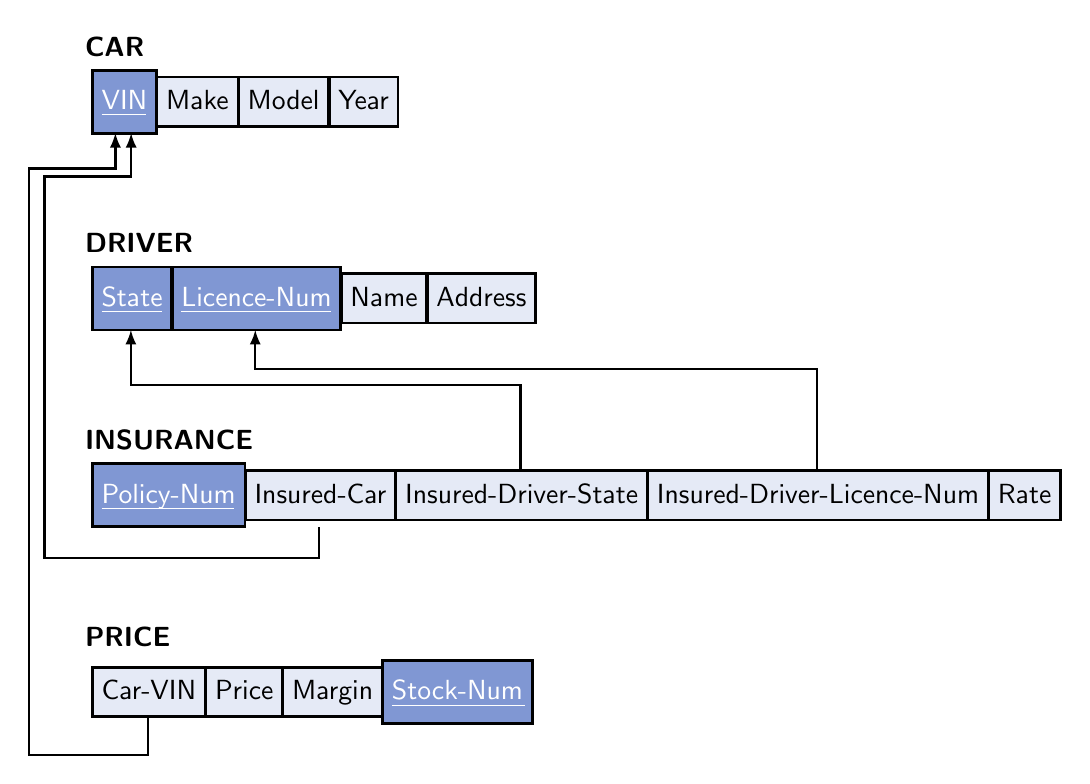
\begin{tikzpicture}[
	PK/.style={% Style for empatized boxes
		rectangle, line width =1pt,
		anchor=west,
		underline, % new property
		align=center,
        text=white,
		minimum height=.8cm,
		text height=1.5ex,
		text depth=.25ex,
        fill=WIRE!50,
		draw=black,
	},
	A/.style={% Style for normal boxes.
		rectangle, 
		line width =1pt,
		anchor=west,
		align=left,
		minimum height=.6cm,
		text height=1.5ex,
		text depth=.25ex,
        fill=WIRE!10,
		draw=black,
		inner ysep=5pt
	},
	underline/.append style={% define new style property
		execute at begin node={%
			\setbox\ubox=\hbox\bgroup
		},
		execute at end node={%
			\egroup\whiteuline{\box\ubox}%
		}
	},
	] % Uff that is all the configuration for tickzpicture xD
	
	% Define an brute force objet "Frame"
	% Variables 1:Position, 2: Identifier, 3: Title of frame 4: Subframe/Boxtype
	\def\Frame(#1)#2[#3]#4{%
		\begin{scope}[shift={(#1)}] 
		\node[font=\bf, anchor=west] (Title) at (-0.2,0.7) {#3}; 
		\edef\k{0}% Variable for box positión
		\edef\x{0}% Variable for named coordinate centering - below box
		\foreach \id/\style in {#4} {%enter sub frame data Name/Boxtype ,Name2/Boxtype | An space before Boxtype is needed 
			\node[\style] (h) at (\k pt,0) {\id}; %  % Draw a node depending on the variables.
			\pgfmathparse{\k+0.5*width{"\id"}+3.4pt} % Uses the textwidth to calculate named coordinate  
			\xdef\x{\pgfmathresult} % The resul is saved in the variable \x
			\draw (\x pt,-0.4) coordinate (\id#2); %Create a named coordinate concatenated: "sub frame data Name"+"identifier"
			\pgfmathparse{\k+width{"\id"}+6.8pt}% Calculate positión for each subframe box.       
			\xdef\k{\pgfmathresult}% Save the value to be added to the next iteration value.
		}    
		\end{scope}
	}% disadvantages: Is not posible to use Frame data Name like: Name_another_desc instead I use Name-another-desc


% CAR(VIN (PK), Make, Model, Year)
% DRIVER(State (PK), Licence-number (PK), Name, Address)
% INSURANCE(Policy-Number (PK), Insured-Car (FK to CAR.VIN), Insured-Driver-State (FK to DRIVER.State), 
% Insured-Driver-Num (FK to DRIVER.Licence-number), Rate)
% PRICE(Stock-number (PK), Car-Vin (FK to CAR.VIN), Price, Margin)

\Frame(0,0){1}[CAR]{
	VIN/PK,
	Make/A,
	Model/A,
	Year/A};

\Frame(0,-2.5){2}[DRIVER]{
	State/PK,
	Licence-Num/PK,
	Name/A,
	Address/A};

\Frame(0,-5){3}[INSURANCE]{
	Policy-Num/PK,
	Insured-Car/A,
	Insured-Driver-State/A,
	Insured-Driver-Licence-Num/A,
	Rate/A};

\Frame(0,-7.5){4}[PRICE]{
	Car-VIN/A,
	Price/A,
	Margin/A,
	Stock-Num/PK};


\draw[FK] % From Insured-Car3 to VIN1
(VIN1)++(0.1,0) -- ++(0,-.55) -- ++(-1.1,0) coordinate (inter)
-- (Insured-Car3 -| inter) -- ++(0,-0.4) coordinate (inter)
-- (Insured-Car3 |- inter) --++(0,0.4);

\draw[FK] % From Car-VIN4 to VIN1
(VIN1)++(-0.1,0) -- ++(0,-.45) -- ++(-1.1,0) coordinate (inter)
-- (Car-VIN4 -| inter) -- ++(0,-0.4) coordinate (inter)
-- (Car-VIN4 |- inter) --++(0,0.5);

\draw[FK] % From Insured-Driver-State3 to State2
(State2) -- ++(0,-.7) coordinate (inter) -- (Insured-Driver-State3 |- inter) --++(0,-1.1);

\draw[FK] % From Insured-Driver-Licence-Num3 to Licence-Num2
(Licence-Num2) -- ++(0,-.5) coordinate (inter) -- (Insured-Driver-Licence-Num3 |- inter) --++(0,-1.3);

\end{tikzpicture}
\end{document}